\subsection{\Glsfmtlong{bart}}

\Gls{bart} est un \gls{llm} de Facebook AI.
Contrairement à \gls{gpt} et \gls{bert}, \gls{bart} est un transformeur \gls{s2s}.
Il utilise \gls{bert} et \gls{gpt} comme encodeur et décodeur respectivement
(voir Figure~\ref{fig.bart}).

\begin{figure}[hbt]
    \centering
    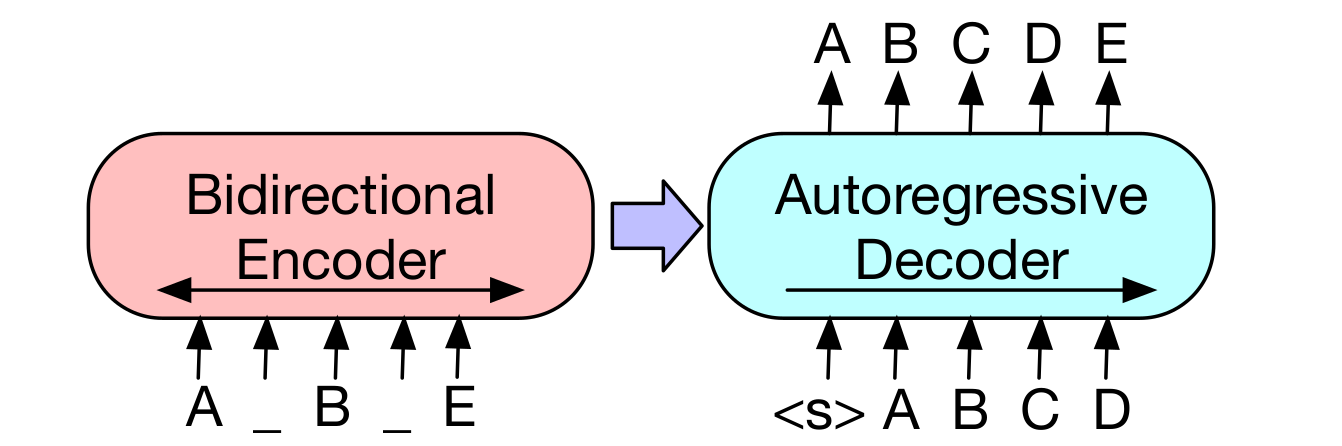
\includegraphics[width=0.8\textwidth]{assets/images/bart.png}
    \caption[Architecture de \glsfmtshort{bart}]
    {Architecture de \glsfmtshort{bart}%
    ~\cite{Lewis_Liu_Goyal_Ghazvininejad_Mohamed_Levy_Stoyanov_Zettlemoyer_2019}.}
    \label{fig.bart}
\end{figure}

À l'instar de \gls{gpt} et \gls{bert}, l'entraînement de \gls{bart} est constitué d'une phase de pré-entraînement
autosupervisé, suivie d'une phase d'affinement.
\gls{bart} est pré-entraîné sur la tâche d'auto-encodage du texte bruité.
Similairement à la \gls{mlm}, un extrait textuel est modifié avant d'être passé à \gls{bart}.
Le modèle est alors chargé de reconstruire le texte original.
Cette tâche est plus difficile que la \gls{mlm}, 
car le but est de reconstruire la séquence plutôt que de prédire les tokens masqués, 
mais aussi, car l'ensemble des modifications possibles est plus grand que l'application d'un masque.
Il inclut également la suppression d'un token (sans le remplacer par \texttt{[MASK]}),
le remplacement d'une suite de token par \texttt{[MASK]} et l'application d'une permutation de phrases%
~\cite{Lewis_Liu_Goyal_Ghazvininejad_Mohamed_Levy_Stoyanov_Zettlemoyer_2019}.

L'affinement dépend de la tâche cible.
\gls{bart} peut être affiné pour les tâches de classification (comme \gls{bert}),
génération de texte (comme \gls{gpt})
ou traduction (voir Figure~\ref{fig.bart-mt}).

\begin{figure}[hbt]
    \centering
    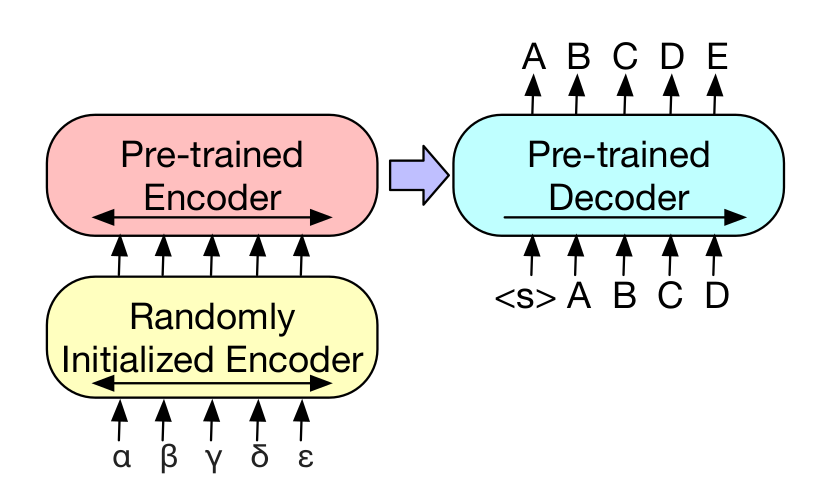
\includegraphics[width=.8\textwidth]{assets/images/bart-mt.png}
    \caption[Affinement de \glsfmtshort{bart} pour la traduction.]
    {Affinement de \glsfmtshort{bart} pour la traduction%
    ~\cite{Lewis_Liu_Goyal_Ghazvininejad_Mohamed_Levy_Stoyanov_Zettlemoyer_2019}.}
    \label{fig.bart-mt}
\end{figure}